\iffalse

%-*- program: xelatex -*-        
%-*- program: biber -*-`        
%-*- program: xelatex -*-
\documentclass[12pt]{article}
\usepackage{amsmath,textcomp,amssymb,geometry,graphicx,enumerate,upquote,color}
\usepackage{hyperref}
\usepackage{float}
\usepackage{tikz}
\usepackage{array}
\usepackage{amsfonts}
\def\Session{Fall 2015}
\usepackage[english]{babel}
\title{Model Selection for the US Indices}
\author{Boying Gong, Xinyue Zhou}
\newenvironment{qparts}{\begin{enumerate}[{(}a{)}]}{\end{enumerate}}
\def\endproofmark{$\Box$}
\newenvironment{proof}{\par{\bf Proof}:}{\endproofmark\smallskip}
\begin{document}
\maketitle

\fi


In this section, we focus on diffrent risk measures under different return frequencies. We're especially interested the behaviour of vaious risk diagnostics under different return frequencies. As we move to longer period such as weekly data, the risk measures such as VaR and ES become unreliable since they are based on the tail of distributions and require a comparatively large amount of dataset. Here we only focused on the comparison of daily and weekly data. 

Figure \ref{fig: mdd_dist_daily_weekly} shows the maximum drawdown distribution of daily (upper panel) and weekly returns (lower panel). Here we use three assets AGG, HYG and TIP as examples. The maximum drawdown distribution of weekly returns are more close to zero and have lighter tails than the distribution of daily returns.

\begin{figure}[h]
\caption{Maximum drawdown (3 month) density of returns based on daily (upper panel) and weekly (lower panel) frequencies} 
\centering 
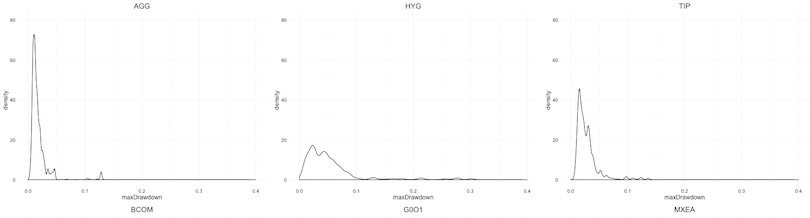
\includegraphics[width=0.9\textwidth]{../figures/maxDrawdown_CED/daily_mdd}
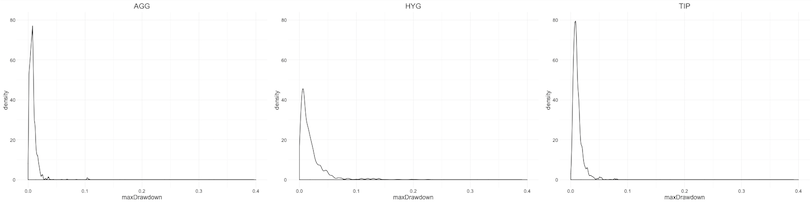
\includegraphics[width=0.9\textwidth]{../figures/maxDrawdown_CED/weekly_mdd}
\label{fig: mdd_dist_daily_weekly}
\end{figure}

We now move to other risk mesures. As we can see from last several sections, ES, VaR and volatility are every closely related. Here I use expected shortfall as an illustration. Figure \ref{fig: ES_daily_weekly_monthly} shows the ES values based on daily (upper panel), weekly (midlle panel) and monthly (lower panel) frequencies. As we expected, there are missing values for the tail mean when we move to longer period such as monthly data. The values of ES of weekly data are nearly as twice as the daily data since they are based on weeekly returns. However, after annualizing the returns, we can see that the number calculated using weekly reeturns are actually smaller. This phenomenon is more obvious when we move to monthly data. The ES calculated using annualized monthly returns are even smaller than its weekly counterpart.

\begin{figure}[h]
\caption{ES (6 month) based on daily (upper panel), weekly (midlle panel) and monthly (lower panel) frequencies} 
\centering 
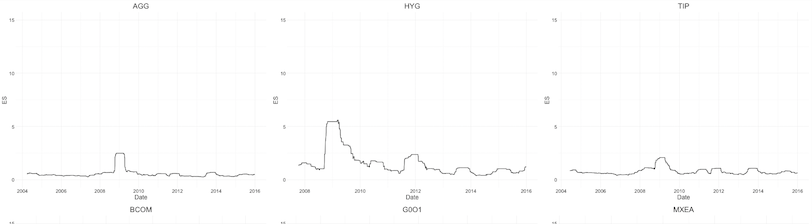
\includegraphics[width=0.9\textwidth]{../figures/rolling_stats/daily_ES}
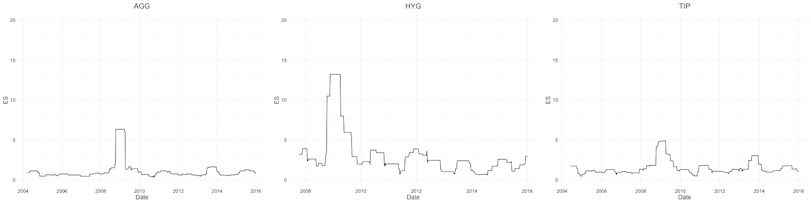
\includegraphics[width=0.9\textwidth]{../figures/rolling_stats/weekly_ES}
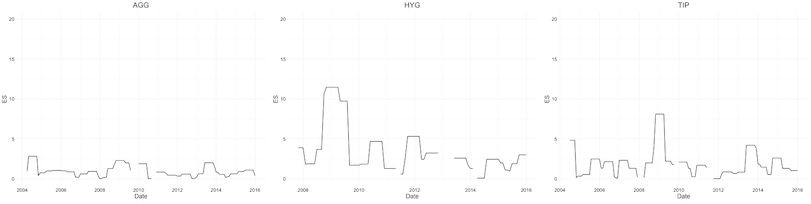
\includegraphics[width=0.9\textwidth]{../figures/rolling_stats/monthly_ES}
\label{fig: ES_daily_weekly_monthly}
\end{figure}



%\end{document}
